%####################################################
% AIBIOM Progress Report
% progress.tex
% author: Carlos Vinhais
% cvinhais@gmail.com 
%####################################################
\documentclass[11pt,a4paper,oneside]{article}

\usepackage{setspace}
%\usepackage[top=3cm,left=3cm,right=3cm,foot=1.5cm,bottom=3cm]{geometry}
\usepackage[top=2cm,left=2cm,right=2cm,bottom=2cm]{geometry}
\usepackage{multicol}
\usepackage{graphicx}
\usepackage{subfigure}
\usepackage{indentfirst}
\usepackage{etoolbox}
\usepackage{indentfirst}
\patchcmd{\thebibliography}{\section*{\refname}}{}{}{}

% Listings:
% -------------------------------------------------------------
\usepackage{listings}								% to list C++ programs
\usepackage{color}
\definecolor{Code}{rgb}{0,0,0}
\definecolor{Decorators}{rgb}{0.5,0.5,0.5}
\definecolor{Numbers}{rgb}{0.5,0,0}
\definecolor{MatchingBrackets}{rgb}{0.25,0.5,0.5}
\definecolor{Keywords}{rgb}{0,0,1}
\definecolor{self}{rgb}{0,0,0}
\definecolor{Strings}{rgb}{0,0.63,0} % green!60!black
\definecolor{Comments}{rgb}{0,0.63,0} % green!60!black
\definecolor{Backquotes}{rgb}{0,0,0}
\definecolor{Classname}{rgb}{0,0,0}
\definecolor{FunctionName}{rgb}{0,0,0}
\definecolor{Operators}{rgb}{0,0,0}
\definecolor{Background}{rgb}{0.99,0.99,0.99}

\lstdefinestyle{customText}{
  %language=Python,
	%belowcaptionskip=1\baselineskip,	
	%frame=single, tabsize=4,
	frame=t, tabsize=4,
	% showspaces=false, showtabs=false, 
	showstringspaces=false,
	backgroundcolor=\color{Background},
  basicstyle=\scriptsize\setstretch{1},
	%commentstyle=\itshape\color{Comments},
}

\lstdefinestyle{customPython}{
  language=Python,
	%belowcaptionskip=1\baselineskip,	
	%frame=single, tabsize=4,
	frame=t, tabsize=4,
	% showspaces=false, showtabs=false, 
	showstringspaces=false,
	backgroundcolor=\color{Background},
  basicstyle=\scriptsize\setstretch{1},
  keywordstyle=\bfseries\color{Keywords},
	commentstyle=\itshape\color{Comments},
  %stringstyle=\color{orange},
	morecomment=[s][\color{Strings}]{"""}{"""},
	morecomment=[s][\color{Strings}]{'''}{'''},
	morecomment=[s][\color{Strings}]{'}{'},
	morekeywords={import,from,class,def,for,while,if,is,in,elif,else,not,and,or,print,break,continue,return,True,False,None,access,as,,del,except,exec,finally,global,import,lambda,pass,print,raise,try,assert},	
}

%####################################################
\begin{document}
%####################################################

% The header file "header.tex" must match  
% the project folder name <observer_dataset>.
% The header file of project folder <1234567_XY0001> must be:
% \def \Observer {1234567} % 7 digits
% \def \Dataset  {XY0001}  % 2 letters + 4 digits
% Header TEX file generated by python script 1.Create_StudentFolders.py 
\def \Observer {1200965}
\def \Dataset  {BG0022}


\begin{flushleft}
	Observer: \textbf{\Observer}\\
	Dataset~: \textbf{\Dataset}\\
	\today
\end{flushleft}

\section*{Manual Segmentation}
% -----------------------------
\begin{figure}[h]
	\centering{
		\subfigure[snapshot0001.png]{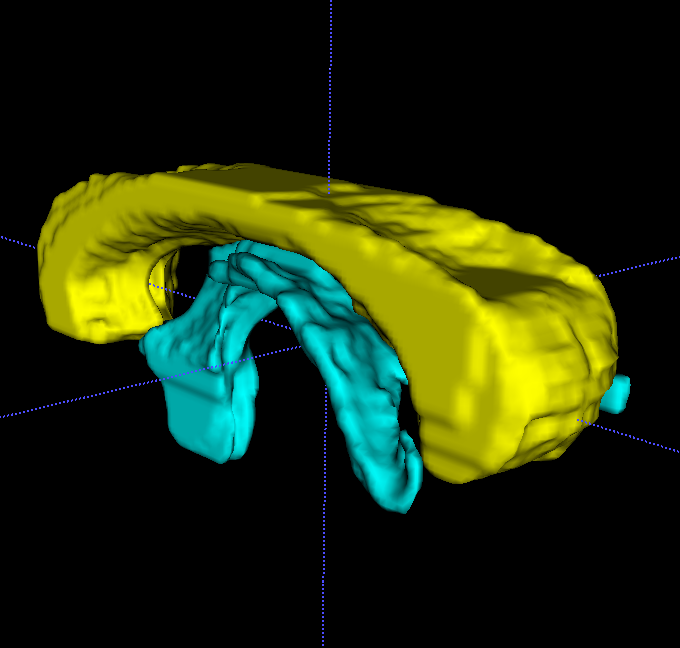
\includegraphics[width=0.4\textwidth]{../itksnap/snapshot0001.png}}
		\subfigure[snapshot0002.png]{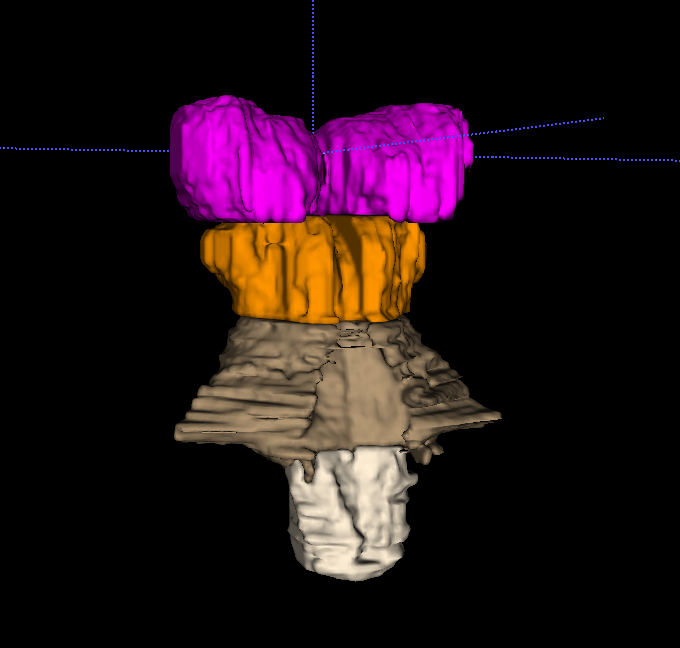
\includegraphics[width=0.4\textwidth]{../itksnap/snapshot0002.png}}
		\subfigure[snapshot0003.png]{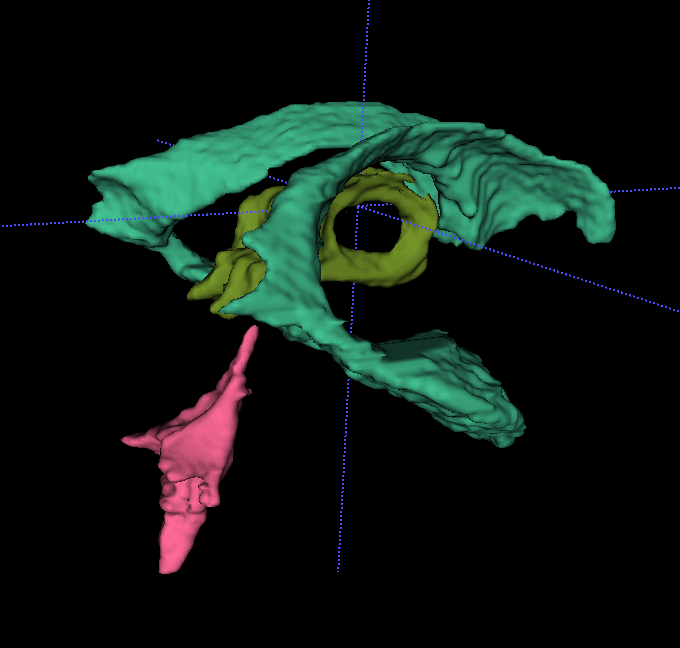
\includegraphics[width=0.4\textwidth]{../itksnap/snapshot0003.png}}
		\subfigure[snapshot0004.png]{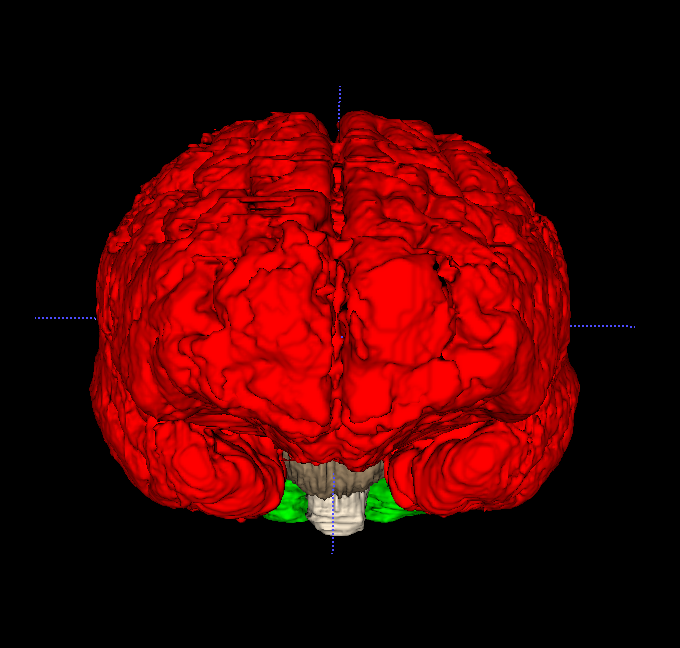
\includegraphics[width=0.4\textwidth]{../itksnap/snapshot0004.png}}
	}
	\caption[itk-SNAP Snapshots]{ \label{fig:Snapshots}
	itk-SNAP: snapshots of 3D views.}	
\end{figure}


\section*{Volumes and Statistics}
% -----------------------------
\lstinputlisting[
style=customText, 
%label={lst:Volumes},
firstline=2, % lastline=5, 
caption={volumes.txt}
]{../itksnap/volumes.txt}

% ==============================
\pagebreak
% ==============================

\begin{flushleft}
Observer: \textbf{\Observer}\\
Dataset~: \textbf{\Dataset}\\
\today
\end{flushleft}


\section*{Resumo}
% -----------------------------
{
	O principal objetivo deste trabalho foi realizar a segmentação manual das estruturas anatômicas de interesse presentes na imagem tridimensional do cérebro humano, fornecida pelo docente. Essa imagem foi adquirida por meio da técnica de angiografia por tempo de voo TOF MRA. Para executar a segmentação, utilizamos o software ITK-Snap, que permitiu a pintura manual de todas as estruturas anatômicas representadas, seguindo as descrições de rotulagem fornecidas no tutorial do ITK-Snap. Esse software é altamente prático e intuitivo, fornecendo todas as ferramentas necessárias para a realização da tarefa com grande eficiência.\cite{py06nimg}
	
	A hidrocefalia é uma das patologias associadas a uma estrutura cerebral estudada, neste caso, os ventrículos cerebrais. Esta doença consiste num acúmulo de líquido excedente nos espaços normais dos ventrículos ou entre as camadas de tecido interna que causa um aumento do crânio e problemas de desenvolvimento. \cite{cruz2022tumor}
	
	Do ponto de vista pessoal, a segmentação manual exigiu bastante esforço, persistência e paciência, tendo sido concluída após várias semanas de trabalho. Devido à imagem fornecida não ser completamente nítida e apresentar ruído em algumas áreas, a segmentação total de algumas estruturas não foi perfeita, no entanto, consegui segmentar todas as estruturas solicitadas, exceto o tronco cerebral (brainstem label), que exigiria a segmentação sobreposta dos labels 7, 8 e 9. Durante a atividade, enfrentei algumas dificuldades, sendo que algumas estruturas foram difíceis de visualizar claramente em todos os planos. Por exemplo, o fórnix foi particularmente desafiador de observar em algumas frames, e os ventrículos laterais foram um pouco complicados devido à sua parte inferior não ser tão visível, o que pode ter resultado em uma dimensão maior do que a real nesta área. Por outro lado, o cerebelo foi facilmente visível em quase todas as frames no plano coronal.
	
	A estrutura que mais demandou tempo foi o cérebro, devido à sua grande dimensão e ao meu desejo de obter um nível detalhado de precisão. Embora o corpo caloso tenha sido mais percetível do que outras estruturas, ainda foi bastante difícil visualizá-lo em algumas frames do plano sagital. No entanto, estou satisfeito com o meu trabalho na segmentação do tronco cerebral (medula, ponte, mesencéfalo), que ficou bastante semelhante às imagens reais que utilizei para comparação. É importante realçar que optei por não conectar o quarto ventrículo ao terceiro ventrículo, uma vez que essa ligação ocorre por meio do aqueduto.\cite{yushkevich2006user}
	
	Apesar das dificuldades na identificação e segmentação das estruturas, a tarefa foi realizada e permitiu uma melhor compreensão da anatomia cerebral de uma forma mais realista e prática. 
 }


\vfill
\section*{Referências}
% -----------------------------

\bibliography{referencias.bib}
\bibliographystyle{ieeetr}


\vfill
%####################################################
\end{document}
%####################################################